\documentclass[a4paper,10pt]{book}

\usepackage[utf8]{inputenc}
\usepackage[T1]{fontenc}
\usepackage[francais]{babel}
\usepackage{lmodern}
\usepackage[top=3cm, bottom=3cm, left=4cm, right=2cm]{geometry}
\usepackage{amsmath}
\usepackage{amsfonts}
\usepackage{amsthm}
\usepackage{amssymb}
\usepackage{mathrsfs}
\usepackage{graphicx}
\usepackage{wrapfig}
\usepackage{stmaryrd}
\usepackage{calrsfs}
\usepackage{xlop}
\usepackage{multicol}
\usepackage{tikz}
\usepackage{circuitikz}
\usepackage[pdftex, pdfauthor={Pierre Gimalac}, pdftitle={Principes de Fonctionnement des Machines Binaires I}, pdfsubject={Informatique}, pdfkeywords={licence, informatique, numération, informatique fondamentale, Java, codage, calcul propositionnel, circuits combinatoires}, colorlinks=true, linkcolor=black, urlcolor=black]{hyperref}
\usepackage{chngpage}
\usepackage{pdflscape}

\newcommand{\R}{\mathbb{R}}
\newcommand{\Rpe}{\mathbb{R}_{+}^{*}}
\newcommand{\N}{\mathbb{N}}
\newcommand{\Z}{\mathbb{Z}}
\newcommand{\C}{\mathbb{C}}
\newcommand{\Q}{\mathbb{Q}}

\begin{document}

\begin{titlepage}
\newgeometry{margin=2.7cm}
\thispagestyle{empty}
\begin{center}
\vspace*{6.7cm}
\Huge \textsc{Principes de Fonctionnement\\
des Machines Binaires I}\\
\vspace{1.5cm}
\Large Pierre Gimalac\\
\vspace{0.5cm}
\large \textit{Licence d'Informatique}
\vfill
\end{center}
\large \textit{Septembre-Décembre 2016}
\hfill 
\large Cours de Jean-Baptiste Yunès
\restoregeometry
\end{titlepage}

\renewcommand{\contentsname}{Sommaire}
\thispagestyle{empty}
\tableofcontents \thispagestyle{empty}

\chapter{Numération}
\section{Principe de la numération positionnelle}
La numération positionnelle est une invention qui nécessita le 0.\\

Dans ce système, la position du chiffre dans le mot modifie sa contribution :\\
\begin{itemize} \item dans « 2 » le '2' représente deux unités, soit $2\times 10^{0}$.
\item dans « 5000 » le '5' représente cinq milliers, soit $5\times 10^{3}$ où 3 est la position à partir de la droite.\\\end{itemize}

On introduit ici le concept de 'base' (ainsi que de sens de lecture) : pour une base entière non nulle, il y a $|b|$ symboles utilisés comme chiffres 0, 1, 2..., b -1.\\

En notation positionnelle de gauche à droite, pour une base b correspondant à un nombre, le \textbf{mot}
$\overline{a_{n-1}a_{n-2}...a_{1}a_{0}}^{b}$ représente le nombre
\begin{center} $\sum\limits_{i=0}^{n-1} a_{i}\times b^{i}$ \end{center}

\textbf{Exemple :}\\
$2859=2*10^{3}+8*10^{2}+5*10^{1}+9*10^{0}$

\section{Base}
\subsection{Définition}
En arithmétique, une base désigne la valeur dont les puissances successives interviennent dans l'écriture des nombres dans la numération positionnelle, ces puissances définissant l'ordre de grandeur de chacune des positions occupées par les chiffres composant tout nombre. Par commodité, on utilise usuellement, pour les bases entières à partir de deux, un nombre de chiffres égal à la base.

\subsection{Bases courantes}
La base la plus couramment utilisée est la base 10 (biologie, mathématiques,...), cependant en informatique les bases les plus courantes sont : \begin{itemize}
\item le binaire (base 2) : 0,1
\item l'octal (base 8) : 0, 1, 2, 3, 4, 5, 6, 7
\item l'hexadécimal : 0, 1, 2, 3, 4, 5, 6, 7, 8, 9, A, B, C, D, E, F\\ \end{itemize}

\section{Conversion d'entiers entre bases}
\subsection{Méthode empirique}
Il s'agit d'une méthode basée sur des approximations successives du nombre (encadrements successifs).

\subsubsection{Exemple}
\begin{center}
\emph{Écrire 167 en base 2 :}\\ \end{center}

\begin{center}
$\begin{array}{rcl} 2^{7}=128\leq &167&<2^{8}=256\\
2^{5}=32\leq &39&<2^{6}=64\\
2^{2}=4\leq &7&<2^{3}=8 \\
2^{1}=2\leq &3&<2^{2}=4 \\
2^{0}=1\leq &1&<2^{1}=2  \end{array}
\begin{array}{rcl}
167-128&=&39\\
39-32&=&7\\
7-4&=&3\\
3-2&=&1\\
1-1&=&0\\ \end{array}$ \end{center}

\begin{center} Alors $(167)_{10}=(10100111)_{2}$ \end{center}

\subsection{Divisions successives}
Cette méthode repose sur le fait que diviser un nombre en base a par un nombre b correspondant à la base finale souhaitée donnera le chiffre des unités dans la base b (à condition d'effectuer les opérations en base a). En répétant l'opération autant de fois que nécessaires (en divisant cette fois le quotient précédemment obtenu), on obtient les nombre en base b (en lisant les restes dans l'ordre inverse).

\subsubsection{Exemple}
Convertir $(1363)_{7}$ en base 10 (donc en base $(13)_{7}$) :\\

$\begin{array}{rcl} (1363)_{7}=&(104)_{7}\times (13)_{7}&+(5)_{7}\\
(104)_{7}=&(5)_{7}\times (13)_{7}&+(3)_{7}\\
(5)_{7}=&(0)_{7}\times (13)_{7}&+(5)_{7}\\\end{array}$
Donc $(1363)_{7}=(535)_{10}$.

\subsection{Recomposition}
Pour passer d'une base $b$ à la base 10, le moyen le plus simple (qui fonctionne en fait pour n'importe quelle base $a$ d'arrivée à condition de faire les calculs en base $a$) est d'utiliser la définition d'un nombre en base $b$ :
\begin{center} $\overline{a_{n-1}a_{n-2}...a_{1}a_{0}}^{b}=\left( \sum\limits_{i=0}^{n-1}a_{i}\times b^{i}\right)_{a}$ \end{center}

\subsubsection{Exemple}
Convertir $(1363)_{7}$ en base 10 :\\\\
$(1363)_{7}=(1\times 7^{3}+3\times 7^{2}+6\times 7^{1}+3\times 7^{0})_{10}=(343+147+42+3)_{10}=(535)_{10}$

\subsection{Méthode de Horner}
On peut utiliser une autre méthode : celle dite de Horner (\textbf{William Georges Horner} \emph{1819-1845}), qui consiste à recomposer le nombre en le lisant de gauche à droite en multipliant chaque chiffre par la base avant de lui ajouter le chiffre suivant et de re-multiplier la base (et cætera).

\subsubsection{Exemple}
Convertir $(1363)_{7}$ en base 10 :\\\\
$(1363)_{7}=(((1\times 7 +3)\times 7 +6)\times 7+ 3)_{10}=(535)_{10}$

\subsection{Relations entre bases}
Le passage entre certaines bases peut être cependant plus simple : si deux base sont telles que l'une est une puissance de l'autre, il suffit alors de 'grouper' ou de 'dégrouper' les chiffres.

\subsubsection{Exemple}
Pour passer de la base 2 à la base 8 on 'groupe' par paquets de trois chiffres binaires.\\
$(110011001100)_{2}=(6314)_{8}$\\

Pour passer de la base 8 à la base 2 on 'dégroupe' en sens inverse.\\
$(1234)_{8}=(1010011100)_{2}$

\subsection{Conversion de non-entiers}
Pour convertir un nombre non entier d'une base $a$ à une base $b$, il faut convertir la partie entière avec les méthodes vues précédemment avant de convertir la partie décimale séparément.\\\\
Pour cela, il faut multiplier la partie décimale (le nombre pris en remplaçant sa partie entière par 0) par la base souhaitée en faisant les opérations dans la base de départ.\\\\
Il faut ensuite noter la partie entière du nombre ainsi obtenu (qui peut être 0) et recommencer l'étape précédente (enlever la partie entière, multiplier par la base d'arrivée,...) jusqu'à obtenir 0.\\

Cependant, un nombre peut ne pas avoir d'écriture finie (si l'on retombe sur un nombre obtenu précédemment c'est que l'écriture est infinie, on note la partie infinie avec un $\omega$ en exposant ou avec une ligne par dessus).

\subsubsection{Exemples}
\begin{itemize}\renewcommand{\labelitemi}{$\bullet$} \item Conversion de $(0,296875)_{10}$ en base 2 :\\

$\begin{array}{rcl}
0,296875\times 2&=&\text{\textbf{0}},593750\\
0,59375\times 2&=&\text{\textbf{1}},18750\\
0,1875\times 2&=&\text{\textbf{0}},3750\\
0,375\times 2&=&\text{\textbf{0}},750\\
0,75\times 2&=&\text{\textbf{1}},50\\
0,50\times 2&=&\text{\textbf{1}},0\\\\
\end{array}$

Donc $(0,296875)_{10}=(0,010011)_{2}$\\\\\\

\item Conversion de $(0,1)_{10}$ en base 2 :\\

$\begin{array}{rcl}
0,1\times 2&=&\text{\textbf{0}},2\\
0,\text{\textit{2}}\times 2&=&\text{\textbf{0}},4\\
0,4\times 2&=&\text{\textbf{0}},8\\
0,8\times 2&=&\text{\textbf{1}},6\\
0,6\times 2&=&\text{\textbf{1}},\text{\textit{2}}\\
\end{array}$ \end{itemize}

Donc $(0,1)_{10}=(0,0(0011)^{\omega})_{2}=(0,0\, \overline{0011})_{2}$

\section{Critères de divisibilité}
\subsection{Preuve par $b-1$}
La preuve par $b-1$ est plus une méthode pour déterminer la validité (ou plutôt la non-invalidité) d'un calcul en base b qu'un critère de divisibilité.\\

Elle consiste à comparer le reste dans la division euclidienne par $b-1$ du résultat du calcul et celui de l'opération réalisée sur les restes par $b-1$ des nombres initiaux (on utilise $b-1$ car peu importe la base, b est congru à 1 modulo $b-1$).\\

Ainsi si les deux restes sont identiques, le résultat n'est pas nécessairement correct mais on sait qu'il ne l'est pas si les deux restes ne sont pas identiques.

\subsubsection{Exemple}
L'opération $1345\times 2345=3154025$ en base 10 :\\

$1345 \equiv 1+3+4+5 (9)$ donc $1345 \equiv 4(9)$.

$2345 \equiv 2+3+4+5 (9)$ donc $2345 \equiv 5(9)$.

$1345\times 2345 \equiv 4*5(9)$ donc $1345\times 2345 \equiv 2(9)$.\\

$3154025 \equiv 3+1+5+4+0+2+5(9)$ donc $3154025 \equiv 2(9)$.\\

L'opération a l'air correcte mais on ne peut réellement savoir si elle l'est de cette manière.

\subsection{Cas général}
Pour déterminer un critère de divisibilité par a dans une base b, il faut regarder avec quoi est congru b (ou ses puissances) modulo a.\\

Ainsi, si la base est un multiple de a, il suffit de vérifier si le chiffre des unités est un multiple de a.

\subsubsection{Exemples}
\emph{Divisibilité de $(31415926535)_{10}$ par 7 :}\\\\
Il faut remarquer que $1000\equiv -1(7)$.\\

On en déduit : $31415926535 \equiv 535-926+415-31(7)$ et donc (après quelques calculs\\
supplémentaires) $31415926535 \equiv 0(7)$.\\\\\\

\emph{Divisibilité de $(31415926535)_{10}$ par 111 :}\\\\
Il faut remarquer que $1000\equiv 1(111)$.\\

On en déduit : $31415926535\equiv 535+926+415+31(111)$ et donc (après quelques calculs\\
supplémentaires) $31415926535 \equiv 20(111)$.

\section{Notations}
\subsection{Écriture scientifique}
La notification scientifique consiste à écrire un réel x sous la forme $a\times 10^{n}$ où\\
$a\in \llbracket 1;10 \llbracket$ et $n\in \N$.

\subsubsection{Exemple}
$65,345$ s'écrit $6,5345\times 10^{1}$.

\subsection{Notation en virgule flottante} \label{flottant}
La notation est une variante de la notation scientifique : elle consiste à écrire un réel x sous la\\
forme $m\times 10^{n}$ où $m\in \llbracket 0,1;1 \llbracket$ et $n\in \N$.
On appelle m la mantisse et n l'exposant.

\subsubsection{Exemple}
$65,345$ s'écrit $0,65345\times 10^{2}$.

\subsection{Écriture des nombres négatifs}
\subsubsection{Utilisation d'un bit de signe}
La notation la plus intuitive des nombres négatifs est d'utiliser un bit (le bit de poids fort en général, il faut donc fixer le nombre de bits) pour indiquer le signe du nombre, ainsi un nombre s'écrit comme son opposé, seul le bit de signe change.

\subsubsection{Exemple}
On cherche l'opposé de 01011101 en base 2 sur 8 bits (avec utilisation d'un bit de signe) : on obtient $11011101$.

\subsubsection{Écriture en complément à $b$}
\emph{On s’intéresse en fait ici uniquement à l'écriture en complément à 2.}\\

Les nombres sont généralement écrits avec une infinité de 0 à gauche, cependant ce n'est pas toujours le cas.\\

Si l'on cherche un nombre positif à ajouter à un autre nombre pour obtenir 0 (donc l'opposé d'un nombre), on se retrouve avec un nombre possédant une infinité de '$1$' sur la gauche (ce que l'on peut considérer comme un nombre négatif).\\

Cette écriture des nombres négatifs est aussi appelée écriture en complément à b (la base du nombre), pour passer d'un nombre à son opposé, il faut remplacer chaque chiffre par son complément à $1$ (le nombre qu'il faut ajouter à ce nombre pour obtenir $1$) puis additionner 1 au nombre obtenu.\\

Cette écriture est celle obtenue en partant de l'écriture naturelle du $0$ et en effectuant des opérations, c'est à dire par exemple qu'enlever 1 à 0 donnera un nombre composé uniquement\\
de 1.

\subsubsection{Exemple}
On cherche l'opposé de 1011101 en base 2 (en écriture en complément à 2) : on arrive sur ${}^{w}(1)0100011$.

\chapter{Numération en machine}
\section{Représentation des nombres en machine}
\subsection{Généralités}
On manipule généralement des nombres relativement petits ou alors des grands nombres avec une précision volontairement faible (on adapte la précision à la taille du nombre).\\

Des choix sont faits pour faciliter l’utilisation des nombres courants : la taille de représentation des nombres est fixée.\\

Sur les ordinateurs on utilise la base 2 qui est plus pratique à utiliser en électronique.

\subsection{Architectures communes}
Aujourd’hui les machines sont couramment à architecture 32 ou 64 bits.\\
Cela signifie entre autres que leur arithmétique interne opère uniquement sur des nombres représentés sur 32 ou 64 bits (respectivement).

\subsection{Lecture des bits}
Il existe plusieurs manière de lire un mot binaire, les principales étant de la gauche vers la droite (bits de poids le plus fort à gauche : \textit{grand indien - grand boutiste - grand boutien - big endian - most significant byte first (MSB)}) et de la droite vers la gauche (bits de poids fort à droite : \textit{petit indien - petit boutiste - petit boutien - little endian - least significant byte first (LSB)}).


\section{Arithmétique sur n bits}
\subsection{Généralités}
Si l'on choisit d'effectuer des opérations sur n bits, on peut représenter $2^{n}$ mots. Le choix est aussi arbitraire que l'on veut mais en pratique on essaie d’établir une correspondance entre les mots binaires et la représentation en base 2 des nombres ; deux représentations sont les plus communes :\\
\begin{itemize}
\item Une représentation non signée des nombres qui permet de représenter les nombres de 0 à $2^{n}-1$ compris.
\item Une représentation signée des nombres qui permet de représenter les nombres de $-2^{n-1}$ à $2^{n-1}-1$ compris (avec un bit de signe).
\end{itemize}

\subsection{Arithmétique modulaire}
\subsubsection{Définition}
Comme dit précédemment, si l'on utilise n bits, seuls $2^{n}$ mots peuvent être représentés, il faudra donc utiliser une arithmétique modulo $2^{n}$.\\

Il s'agit de l’arithmétique dans laquelle on ne s’intéresse pas aux nombres eux-mêmes mais à leurs restes par la division euclidienne dans l’arithmétique modulo p (pour p fixé), les nombres $i+kp$ (avec $0\leq i<p$) sont tous équivalents.\\

\subsubsection{Calculs}
Dans une arithmétique modulaire, les calculs peuvent provoquer un échappement de retenue ou l'entrée d'une retenue.\\

On fait ainsi la différence entre un résultat dans l'arithmétique ordinaire et dans l'arithmétique modulaire (dans laquelle un produit de nombres positifs peut donner un nombre négatif, une somme de positifs peut donner un négatif,...).\\

\textbf{Exemple}\\

Sur 3 bits, l'opération $111+010$ : $111+010=001$.\\
L'opération est correcte modulo 8 ($2^{3}$) mais pas dans l'arithmétique ordinaire.

\subsubsection{Utilisation de la notation en complément à $2$}
Pour simplifier les calculs, on utilise la représentation des entiers en complément à b (ici b=2).\\
Cette représentation permet de simplifier certaines opérations arithmétiques.\\

\subsubsection{Détection d'erreurs}

Dans l'arithmétique modulaire, les grands nombres sont 'réduits' à leur reste modulo. Le repérage des erreurs dépend de si l’on fait de l’arithmétique signée ou non.\\

Pour l’arithmétique non signée il suffit d’observer la retenue qui 'sort' :\\
\begin{itemize} \item Pour l’addition c’est la retenue sortante.
\item Pour la soustraction c’est la retenue entrante.\\ \end{itemize}
Si la retenue en question est 1, il y a une erreur, sinon l’opération est correcte.\\\\\\

Pour l’arithmétique signée il suffit d’observer les signes des opérandes et du résultat :\\
\begin{itemize} \item Pour l’addition additionner deux nombres positifs ne peut pas donner un nombre négatif et additionner deux négatifs ne peut donner un positif.
\item Pour la soustraction soustraire un positif à un négatif ne peut donner un positif et soustraire un négatif à un positif ne peut donner un négatif.\\ \end{itemize}
Il suffit donc d’observer les signes.

\section{Types de nombre}
\subsection{Introduction}
Chaque langage définit des types permettant de réaliser des calculs arithmétiques.\\

Le type d’une variable permet de fixer sa taille en mémoire, l’interprétation du mot binaire correspondant ainsi que l’ensemble des opérations légales et leur sémantique.\\

Connaître les types de variables est donc très important pour éviter d'éventuelles erreurs.\\\\
En effet, si les machines détectent en interne les erreurs arithmétiques, la plupart des langages de programmation ne répercutent pas celles-ci à l’utilisateur.

\subsubsection{Exemples}
En java, les types de nombres sont \textit{byte, short, int, long, float, double, double, char} :\\

\begin{itemize}\renewcommand{\labelitemi}{$\bullet$}
\item \textit{byte} permet la représentation signée en complément à 2 d'entiers sur 8 bits.
\item \textit{short} permet la représentation signée en complément à 2 d'entiers sur 16 bits.
\item \textit{int} permet la représentation signée en complément à 2 d'entiers sur 32 bits.
\item \textit{long} permet la représentation signée en complément à 2 d'entiers sur 64 bits.
\item \textit{float} permet la représentation signée des non-entiers sur 32 bits.
\item \textit{double} permet la représentation signée des non-entiers sur 64 bits.
\item \textit{char} permet la représentation des caractères (de leur code Unicode) sur 16 bits.
\end{itemize}

\subsection{Expressions avec différents types}
\subsubsection{Affectation}

Si le nombre peut être représenté dans le type d'arrivée, il n'y a pas de problème, il se produit une \emph{promotion} qui est une opération implicite car non-dangereuse.\\

La promotion consiste simplement en l’extension du signe : on complète à gauche avec le signe de la valeur à compléter.\\

\textbf{Rappel :} les positifs ont une infinité de 0 à gauche, les négatifs une infinité de 1 à gauche.\\\\

L'opération inverse se produit quand le nombre ne peut pas être représenté dans le type d'arrivée, cette opération appelée cast, conversion ou encore coercition doit être explicite (en Java).\\

Dans le cas d'un passage d'un type entier à un autre, les derniers bits sont gardés (le nombre est donc exact dans l'arithmétique modulaire mais ce n'est pas forcément le même).

\subsubsection{Opérations}

En java, c'est toujours le plus grand type qui l'emporte mais les opérations sont au moins réalisées en \emph{int}.\\
La priorité des types est : \emph{byte < short < int < long < float < double}\\

Si l'opération ne peut être faite naturellement (par exemple si l'on veut mettre une somme de \textit{short} dans un \textit{short}), il faut préciser explicitement le type d'arrivée avant l'opération.

\subsubsection{Exemples}

\textit{short + short }$\mapsto$ converti en \textit{int + int }$\mapsto$ \textit{int}.

\textit{short * int }$\mapsto$ converti en \textit{int * int }$\mapsto$ \textit{int}.

\section{Écriture de nombres en JAVA}
\subsection{Écriture des nombres dans d'autres bases}
\subsubsection{Décimal}
Il s'agit d'une suite de chiffres de $0$ à $9$ (éventuellement précédées d'un signe $+$ ou $-$) dont le premier chiffre n'est pas un $0$.\\

\textbf{Exemple}\\
On peut noter 31415 pour un nombre décimal.

\subsubsection{Octal}
Il s'agit d'une suite de chiffres de $0$ à $7$ (éventuellement précédées d'un signe $+$ ou $-$) dont le premier chiffre est un $0$.\\

\textbf{Exemple}\\
On peut noter 031415 pour un nombre octal.

\subsubsection{Hexadécimal}
Il s'agit d'une suite de chiffres de $0$ à $9$ et de lettres de A à F (éventuellement précédées d'un signe $+$ ou $-$) et précédée de $0$x.\\

\textbf{Exemple}\\
On peut noter 0x3EF pour un nombre hexadécimal.

\subsubsection{Binaire}
Il s'agit d'une suite de $0$ et de $1$ (éventuellement précédées d'un signe $+$ ou $-$) et précédée de $0$b.\\

\textbf{Exemple}\\
On peut noter 0b011001100101 pour un nombre binaire. 

\subsection{Écriture de certains types}
\subsubsection{Float}
Les float doivent être écrits avec le suffixe 'f'.

\subsubsection{Double}
Les double doivent être écrits avec le suffixe 'd'.

\subsubsection{Long}
Les longs doivent être écrits avec le suffixe 'l' ou 'L'.

\newpage

\section{Opérations particulières}
\subsection{Division '$/$'}
Pour des types entiers, la division de a par b renvoie le quotient de la division de |a| par |b|.

\subsection{Reste '$\%$'}
Pour des types entiers, le reste de la division de a par b renvoie a-b*(|a|/|b|) (le reste peut donc ici être négatif).

\subsection{Décalage}
En binaire, multiplier par une puissance de 2 revient à ajouter un certains nombres de 0 à droite et diviser par une puissance de 2 revient à enlever un certains nombre de bits sur le droite.\\

Les opérations correspondantes sur les mots sont appelées décalage vers la gauche et vers la droite.\\

En java elles se notent à l’aide des opérateurs $<<$, $>>>$ et $>>$. Leur argument est le nombre de décalages unitaires (donc la puissance de 2 utilisée comme multiplicateur ou diviseur).

L'opération $>>>$ ne conserve pas le bit de signe (elle rajoute toujours des 0 à gauche du nombre) alors que $>>$ conserve le bit de signe (si le nombre est négatif, elle rajoute des 1 à gauche et elle rajoute des 0 pour un nombre positif).\\\\\\

\textbf{Exemples (sur 8 bits)}\\

$10101010 >> 2 = 11101010$

$10101010 >>> 4 = 00001010$

$00110011 << 3 = 10011000$

\newpage

\section{Notation des réels}
\subsection{Écriture générale}
Il existe des normes pour représenter les flottants (écriture en virgule flottante, voir page \pageref{flottant}):\\
on utilise un bit de signe, 8 ou 11 bits pour l'exposant selon si l'on est en simple précision sur 32 bits ou en double précision sur 64 bits et enfin 23 ou 52 bits pour la mantisse (les chiffres se situant après le tout premier 1 dans l'écriture en base 2).\\

L'exposant en binaire s'obtient en additionnant à '01111111' (en simple précision) la puissance en base 2 de 2 dans l'écriture scientifique.

\subsubsection{Exemple}
Écrire 5,34375 en notation flottante :\\

$(5,34375)_{10}=(101,01011)_{2}=(1,0101011\times 10^{10})_{2}$.\\\\
L'exposant est donc $01111111+10=10000001$ et la mantisse est $0101011$

donc en flottant $5,34375$ s'écrit $01000000101010110000000000000000$.

\subsection{Valeurs particulières}
\subsubsection{Le zéro}
Tous les bits sont égaux à 0, seul le signe peut varier.

\subsubsection{L'infini}
La mantisse est nulle, le bit de signe est celui de l'infini et les bits de l'exposant sont à 1.

\subsubsection{NaN}
Les bits de l'exposant sont à 1, mais contrairement à l'infini ici la mantisse est non nulle

\subsection{Remarque}
Certains nombres ne sont pas représentables avec cette notation, on se sert donc d'arrondis. De ce fait, il faut éviter de comparer deux flottants qui pourraient différer uniquement à cause de l'arrondi.

\chapter{Codage et compression}
\section{Introduction}
\subsection{Définition}
Le codage est la conversion d'une représentation en une autre. Le codage peut aller de pair avec la numérisation, un procédé consistant à transformer un signal (généralement analogique) en une représentation discrète.

\subsection{Objectifs}
Le codage est utilisé à différentes fins :\\ \begin{itemize}
\item Représenter quelque chose dans un système numérique.
\item Économiser de l’espace (compression de données).
\item Rendre illisibles aux non initiés des données (cryptographie).
\item Résister aux altérations, pertes ou mutations (codes correcteurs).\\ \end{itemize}

En informatique, il s'agit surtout de coder l'information sous forme de 0 et de 1 pour qu'elle soit compréhensible par un ordinateur.

\newpage

\section{Théorie des codes}
\subsection{Code de longueur variable}
\subsubsection{Principe}
Il est possible de coder des mots avec un code de longueur variable, le problème étant qu'il faut s'assurer que le codage est décodable sans ambiguïté.

\subsubsection{Exemples}
Soit t un codage. t(a)=00, t(b)=11, t(c)=111110. Ce codage est bon car il ne peut y avoir de doute au moment du décodage.\\

Soit g un autre codage. g(a)=0, g(b)=01, g(c)=10. Ce codage n'est pas bon car il y a des situations où l'on ne peut savoir qu'est-ce qui a été codé (par exemple si le codage est 010 on ne peut savoir si 'ac' ou 'ba' a été codé).\\

Le morse est un codage de longueur variable.

\subsection{Code de longueur fixe}
\subsubsection{Principe}
L'inconvénient des codes de longueur fixe est que si les mots à coder sont nombreux, le code peut devenir très long (il faut utiliser un nombre n de bits par mot tel que $2^{n}\geq k$ avec k le nombre de mots à coder).\\

En général, pour un nombre de mots à coder A, et avec un nombre B de caractères dans le code d'arrivée (en général 2 : 0 et 1), il faut coder chaque caractère sur un nombre k de caractère tel que k$\geq \log_{\text{B}}$(A).

\subsubsection{Exemple}
Le codage des nombres sur 8 bits est un codage de longueur fixe, chaque nombre est un enchaînement de 8 bits et il ne peut y avoir de doute sur le nombre représenté.

\newpage

\section{Codage d'une image}
\subsection{Principe}
On décompose l’image en points dont la valeur est la composition des valeurs des caractéristiques intéressantes (en général la couleur).

\subsection{Codage des couleurs}
Les dispositifs de reproduction de la couleur ne peuvent représenter l’ensemble des couleurs que l’œil humain peut percevoir. L’ensemble des couleurs reproduites par un appareil donné est son gamut.\\

Il existe de nombreuses façons de coder les couleurs numériquement, les principales étant en noir et blanc, en niveaux de gris et en RVB, un système additif qui compose une couleur par addition de couleurs primitives (rouge, vert, bleu).\\

La valeur associée à un pixel représente : \begin{itemize} 
\item soit une valeur « directe ».
\item soit une indirection dans une table qui contient les valeurs (color table).\\ \end{itemize}

Codage d'une couleur RGB en mode direct : un nombre pour le R, un pour le V, un pour le B.\begin{enumerate}
\item mode arithmétique avec des valeurs décimales entre 0 et 1.
\item mode pourcentage avec des valeurs (entières ou non) entre 0\% et 100\% .
\item mode numérique avec un nombre sur n-bits. \end{enumerate}

\subsection{Caractéristiques d’une image}
La définition de l’image correspond au nombre de lignes et de colonnes de pixels.\\

La résolution correspond à la finesse de l’image, c'est-à-dire au nombre de pixel par unité de mesure (densité linéaire). Elle est en général exprimée en pixel par pouce (ou point par pouce).\\

Le nombre de bits utilisés pour coder une image est appelé son poids. Sans compression, c’est le produit de la définition par le nombre de bits utilisés pour coder un pixel.

\subsection*{Remarque}
Il a existé par le passé des dispositifs d’affichage vectoriel : téléviseurs cathodiques, écrans vectoriel. Il existe encore certains appareils de mesure de ce type comme les oscilloscopes.

\subsection{Compression}
Il est possible de gagner de l'espace en compressant une image, dans la plupart des cas cela va provoquer une perte de précision mais pas toujours.\\

Si l'on veut coder une image faite de pixels noirs et blancs (un texte par exemple), on peut ne coder que la longueur des suites de pixels noirs et de pixels blancs, ce qui permet d'économiser de l'espace (on peut combiner cette méthode avec le code de Huffman, voir page \pageref{Huffman}, pour plus d'efficacité).\\

Il est aussi possible de compresser une image de manière à réduire sa qualité (donc son nombre de pixels) et donc sa taille en mémoire.

\newpage

\section{Codage d'un signal}
\subsection{Numérisation}
\subsubsection{Définition}
La numérisation désigne le processus consistant à convertir un signal analogique en données numériques.\\

Il fait appel à l’échantillonnage qui consiste à sélectionner dans un ensemble un nombre fini d’éléments considérés
comme représentatifs. L’échantillonnage est une approximation.\\

Il fait appel à la quantification qui consiste à associer à chaque élément prélevé une valeur numérique discrète.\\

Ces deux paramètres conditionnent la qualité d’approximation et donc de la reproduction du signal original.\\

L’échantillonnage est très généralement effectué à intervalles réguliers et est alors mesuré en Hertz. La finesse de la quantification est mesurée en bits.

\begin{center} 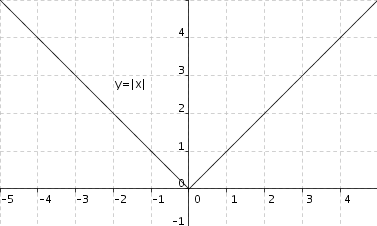
\includegraphics[scale=0.6]{images/004.jpg} \end{center}

\subsubsection{Théorème de Nyquist-Shannon}
La reconstitution approximative d’un signal analogique depuis sa forme numérisée nécessite une fréquence d’échantillonnage au moins deux fois plus élevée que la largeur de la bande.

\subsection{Compression}
Il s’agit ici d’obtenir une représentation plus compacte pour transmettre l'information (économie de bande passante) ou pour stocker (économie d’espace).\\

Il existe deux types de compression :\\ \begin{enumerate}
\item conservative ou sans perte : le message originel peut-être reconstruit à l’identique en inversant la fonction, ce type de compression est recherché avec du texte par exemple.
\item non conservative ou avec perte : le message originel n’est pas reconstruit à l’identique, mais un
message similaire est obtenu à l’inversion, c'est souvent le cas des images et des sons. Cette compression permet d’obtenir de très bons taux de compression. \end{enumerate}

\section{Code de Huffman} \label{Huffman}
\subsection{Principe}
Le principe du codage de Huffman est de coder avec des mots de petite longueur les lettres les plus fréquentes et de coder avec des mots de plus grande longueur les lettres les moins fréquentes, il s'agit donc un codage de longueur variable.\\

\subsection{Arbre de Huffman}
Pour obtenir un codage à partir des fréquences des lettres, on va fabriquer un arbre.\\
C’est une structure dans laquelle on trouve des nœuds : un nœud permet de désigner d’autres nœuds ; s'il ne désigne rien on l'appelle une feuille, s'il est sans ascendant on l'appelle racine.\\

Ici l'arbre est binaire (avec uniquement des nœuds à deux descendants), les feuilles représentent les lettres et leur fréquence associée, les nœuds représentent la somme des fréquences des lettres qu’ils désignent.\\

Pour fabriquer cet arbre on part des arbres réduits aux simples lettres. À chaque étape, on sélectionne deux arbres dont les fréquences des racines sont les plus petites et on fabrique un arbre dont le nœud racine pointera vers les deux arbres sélectionnés et dont la fréquence sera simplement la somme des fréquences.

\subsubsection{Exemple}
La fréquence des lettre est A:8, B:7, C:5, D:3, E:1.
\begin{center} \begin{tikzpicture}[scale=1]

\draw[>=latex,->,thick] (1.5,2.5) -- (0.33,0.66) node[near end,above left] {$0$} ;
\draw[>=latex,->,thick] (1.5,2.5) -- (2.67,0.66) node[near end,above right] {$1$} ;
\draw[>=latex,->,thick] (10.5,2.5) -- (9.33,0.66) node[near end,above left] {$0$} ;
\draw[>=latex,->,thick] (10.5,2.5) -- (11.67,0.66) node[near end,above right] {$1$} ;
\draw[>=latex,->,thick] (7.5,4) -- (6.33,0.66) node[midway,left] {$0$} ;
\draw[>=latex,->,thick] (7.5,4) -- (9.85,2.85) node[near end,above] {$1$} ;
\draw[>=latex,->,thick] (4.5,5.5) -- (6.836,4.348) node[near end,above] {$1$} ;
\draw[>=latex,->,thick] (4.5,5.5) -- (2,3.05) node[midway,above left] {$0$} ;

\fill[color=blue!60] (0,0) circle (0.75) ;
\node at (0,0) {A:8} ;
\fill[color=blue!60] (3,0) circle (0.75) ;
\node at (3,0) {B:7} ;
\fill[color=blue!60] (6,0) circle (0.75) ;
\node at (6,0) {C:5} ;
\fill[color=blue!60] (9,0) circle (0.75) ;
\node at (9,0) {D:3} ;
\fill[color=blue!60] (12,0) circle (0.75) ;
\node at (12,0) {E:1} ;
\fill[color=blue!60] (1.5,2.5) circle (0.75) ;
\node at (1.5,2.5) {:15} ;
\fill[color=blue!60] (10.5,2.5) circle (0.75) ;
\node at (10.5,2.5) {:4} ;
\fill[color=blue!60] (7.5,4) circle (0.75) ;
\node at (7.5,4) {:9} ;
\fill[color=blue!60] (4.5,5.5) circle (0.75) ;
\node at (4.5,5.5) {:24} ;

\end{tikzpicture} \end{center}

Le codage de A est donc 00, le codage de B est 01, le
codage de C est 10, celui de D est 110 et celui de E est
111.\\

Ici les lettres les plus fréquentes sont codées sur 2 bits et
les plus rares sur 3. Un codage ordinaire (de longueur fixe) aurait conduit à utiliser 3 bits par
lettre.\\

Codons 'ABCDABCABAEBCADABCDBACBA' (message qui respecte strictement la fréquence des lettres):
'0001101100001100001001110110001100001101100100100100'.\\

52 bits ici contre 75 avec un codage de longueur fixe, ce qui donne une économie d'environ 33\%.

\section{Cryptographie}
\subsection{Exemples de méthodes de chiffrement}
\subsubsection{Chiffre de César}
Cette méthode de codage repose sur une permutation circulaire de l’alphabet. Les lettres sont décalées de p (pour un p choisi) rangs dans l’ordre alphabétique. Ce codage est facilement déchiffrable par analyse de la fréquence des lettres ou encore par la méthode brute (il n'y a que 25 possibilités).

\subsubsection{Chiffre de Vigenère}
Le chiffre de Vigenère repose sur l'utilisation du chiffre de César et d'un texte (la clé) dont chaque lettre va déterminer le nombre de rang dont on va décaler la lettre à coder (la clé est répétée tout le long du texte à coder).

\subsubsection{Chiffre de Vernam}
Un chiffre de Vigenère pour lequel la clé est aussi longue que le texte, obtenue par distribution aléatoire et ne doit être employé qu’une seule fois.\\
Si les conditions sont réunies, le chiffre est inviolable.

\subsubsection{Le RSA}
Le chiffrement RSA est asymétrique, il repose sur un système de clés publique et privée et sur l'utilisation de grands nombres premiers pour coder un message (trop compliqué à expliquer en détail).

\subsection{Contrôle d'erreur}
Pour contrôler la présence d'erreurs, il existe plusieurs méthodes.\\

La plus simple est simplement de répéter le message, mais il en existe des plus complexes permettant de repérer la présence d'une erreur (deux erreurs peuvent se compenser) : l'ajout d'un bit de contrôle en fonction de la parité par exemple.\\

\subsubsection{Code de Hamming (7,4)}
Le code de Hamming rajoute plusieurs bits vérifiant les parités de plusieurs morceaux du code et permettant même de repérer une erreur assez précisément : si un bit de contrôle change, alors il est l'erreur, si deux changent alors c'est un bit du code qui est l'erreur,...\\

Son principe est le suivant : si l'on veut coder une suite de bits, on la sépare en 'paquets' de
$\begin{array}{rcl}\text{4 bits }d_{1}d_{2}d_{3}d_{4}. \text{ Les }p_{i}\text{ bits de contrôle sont tels que }&-&p_{1}\text{ est la somme de contrôle de }d_{1}+d_{4}+d_{2}.\\
&-& p_{2}\text{ est la somme de contrôle de }d_{1}+d_{4}+d_{3}.\\
&-&p_{3}\text{ est la somme de contrôle de }d_{2}+d_{4}+d_{3}.\\\\ \end{array}$

Les bits ainsi obtenus sont $p_{1}p_{2}p_{3}d_{1}d_{2}d_{3}d_{4}$ dans le cas du code de Hamming (7,4).

\begin{center} 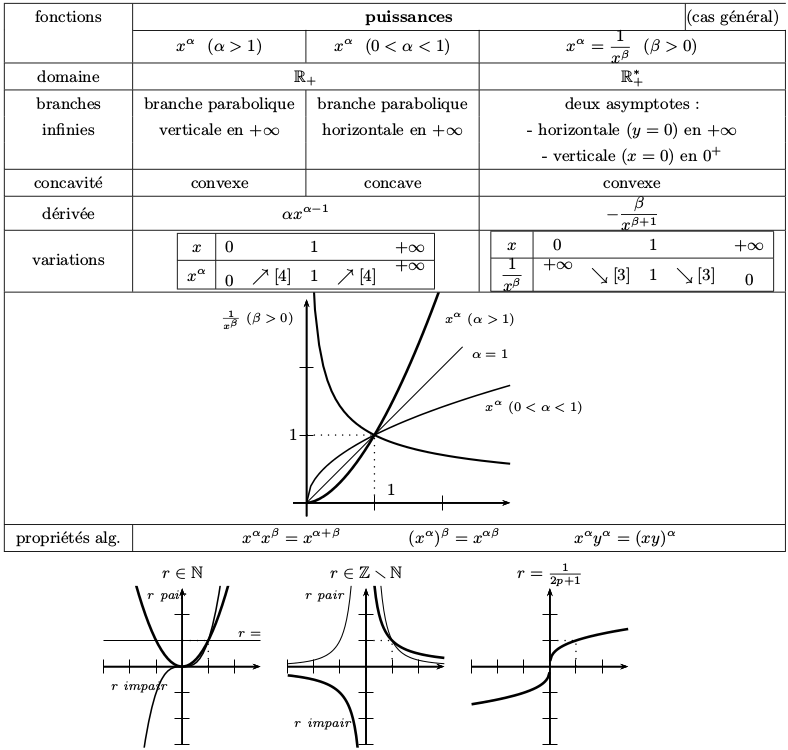
\includegraphics[scale=0.3]{images/005.png} \end{center}

\chapter{Calcul propositionnel}
\section{Introduction}
\subsection{Définition}
Le calcul propositionnel ou calcul des propositions est une théorie logique qui formalise le raisonnement logique.\\

Le calcul propositionnel ne se préoccupe que de la bonne articulation logique des propositions entre elles pas de leur vérité intrinsèque.\\

\subsection{Algèbre de Boole}
L’algèbre de Boole est le calcul des propositions dont le domaine est celui des booléens B, l’ensemble a deux éléments \{ FAUX, VRAI \}, \{ false, true \} ou \{ 0, 1 \} qu’on appelle valeurs de vérité.\\

Une proposition est une entité qui donne une information à propos d’un état des choses.

\subsection{Notations}
Il existe deux symboles destinés à représenter les valeurs de vérité :\\\\
$\top$ (Top) : VRAI\\
$\bot$ (Bottom) : FAUX\\

Certains langages comme JAVA notent la valeur de vérité avec des variables appelées \textbf{Booléen} pouvant prendre deux valeurs littérales : \textit{true} et \textit{false}.

\section{Opérateurs logiques}
\subsection{Généralités}
Les connecteurs (ou opérateurs) permettent de construire des propositions plus élaborées.\\

Les principaux connecteurs sont \textbf{et} et \textbf{ou}, qui attribuent respectivement la valeur de vérité de l'intersection des deux propositions (renvoie vrai si les deux le sont) et la valeur de vérité de l'union des deux propositions (renvoie vrai si au moins un des deux est vrai).\\

Les connecteurs n-aires sont des applications de \textbf{B}$^{n}\mapsto$\textbf{B} (avec \textbf{B}=\{\textit{true}, \textit{false}\}).

\subsection{Notations}
Il y a diverses notations pour les connecteurs logiques (\textbf{Java}) :
\begin{description}
\item[\textit{et} :] p and q, p$\wedge$q, p.q, p$\&\&$q, \textbf{p\&q}
\item[\textit{ou} :] p or q, p$\vee$q, p+q, p||q, \textbf{p|q}
\item[\textit{x-ou} :] p xor q, p$\oplus$q, \textbf{p\^{}q}
\item[\textit{n-et} :] p nand q, p$\barwedge$q
\item[\textit{n-ou} :] p nor q, p$\veebar$q
\item[\textit{équivalence} :] p si et seulement si q, p$\Leftrightarrow$q, p$\equiv$q, \textbf{p==q}
\item[\textit{implication} :] si p alors q, p$\Rightarrow$q, p$\supset$q
\end{description}

\subsection{Connecteurs n-aires}
Il y a 4 connecteurs unaires : absurdisation, identité, négation, tautologisation.
\begin{center} 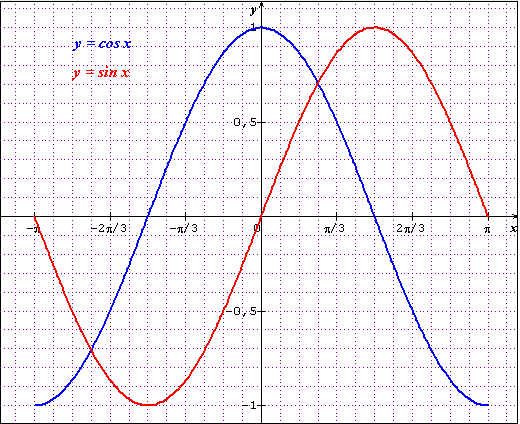
\includegraphics[scale=0.45]{images/001.png} \end{center}

Il y a 16 connecteurs binaires.
\begin{center} 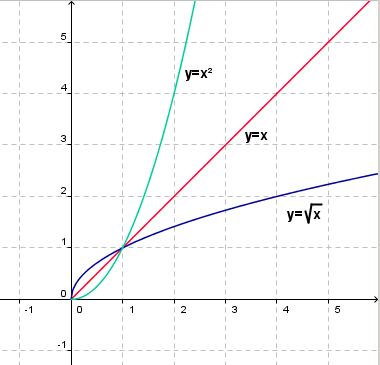
\includegraphics[scale=0.45]{images/002.png} 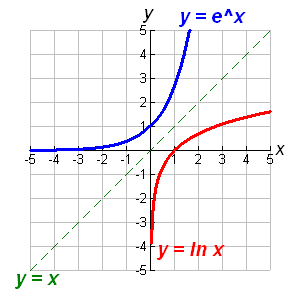
\includegraphics[scale=0.4475]{images/003.png}\end{center}

\begin{wrapfigure}[10]{r}{0.5cm} \begin{tikzpicture}
\draw (0,0) -- (-0.5,-1) ;
\node at (-0.55,-1.2) {$\vee$} ;
\draw (0,0) -- (0.5,-1) ;
\node at (0.55,-1.2) {c} ;
\draw (0,1) -- (0,0.4) ;
\node at (0,0.2) {$\wedge$} ;
\node at (0,1.1) {$\neg$} ;
\draw (-0.55,-1.5) -- (-1.05,-2.5) ;
\draw (-0.55,-1.5) -- (-0.05,-2.5) ;
\node at (-1.05,-2.7) {a} ;
\node at (-0.05,-2.7) {b} ;
\end{tikzpicture} \end{wrapfigure}

\section{Représentations}
\subsection{Arbre de vérité}
Il est parfois pratique d’associer à une formule son arbre syntaxique qui reflète sa structure profonde. Ainsi pour $\neg$((a $\vee$ b) $\wedge$ c) on obtient l'arbre de droite.\bigskip

L'arbre syntaxique exprime la formule indépendamment de sa syntaxe formelle. La forme infixe nécessite des parenthèses $\neg$((a $\vee$ b) $\wedge$ c) alors que les formes préfixe et postfixe (où l'on lit l'arbre en partant du haut, en le longeant par la gauche et en notant quand on passe respectivement à gauche ou droite d'un opérateur ou d'une variable) n'en nécessitent pas.\\

La forme préfixe de cette formule est donc $\neg\wedge\vee$abc alors que sa forme postfixe est ab$\vee$c$\wedge\neg$.

\subsection{Table de vérité}
Il est fréquent de présenter les valeurs d’une expression sous la forme d’une table où les entrées sont les valeurs des variables de l’expression et les sorties la valeur de l’expression.

\subsubsection{Exemple}
Pour la formule E$_{1}$=(((a$\Rightarrow$ ($\neg$b))$\vee$($\neg$(b$\Leftrightarrow$c)))$\wedge$(a$\oplus$c):\\\\
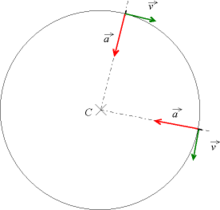
\includegraphics[scale=0.4]{images/006.png}

\subsection{Propriétés des opérateurs logiques}
\begin{itemize}\renewcommand{\labelitemi}{$\bullet$} \item La négation est involutive : $\neg\neg$a$\Leftrightarrow$a.\\
\item Les connecteurs $\wedge$ et $\vee$ sont idempotents, c’est-à-dire que a$\vee$a$\Leftrightarrow$a et a$\wedge$a$\Leftrightarrow$a.\\
\item Il existe aussi des simplifications fondamentales :\\
a$\vee\bot\Leftrightarrow$a, a$\vee\top\Leftrightarrow\top$, a$\vee$($\neg$a)$\Leftrightarrow\top$\\
a$\wedge\bot\Leftrightarrow\bot$, a$\wedge\top\Leftrightarrow$a, a$\wedge$($\neg$a)$\Leftrightarrow\bot$\\
\item Absorption : (a$\wedge$b)$\vee$a$\Leftrightarrow$a, (a$\vee$b)$\wedge$a$\Leftrightarrow$a.\\
\item Distributivité : \\
de $\vee$ par rapport à $\wedge$ : a$\vee$(b$\wedge$c)$\Leftrightarrow$(a$\vee$b)$\wedge$(a$\vee$c), a+\\
(b.c)$\Leftrightarrow$(a+b).(a+c)\\
de $\wedge$ par rapport à $\vee$ : a$\wedge$(b$\vee$c)$\Leftrightarrow$(a$\wedge$b)$\vee$(a$\wedge$c), a.\\
(b+c)$\Leftrightarrow$(a.b) + (a.c)\\
\item loi de De Morgan
$\neg$(a$\vee$b)$\Leftrightarrow\neg$a $\wedge$ $\neg$b
$\neg$(a$\wedge$b)$\Leftrightarrow\neg$a $\vee$ $\neg$b\\

\item Priorité des principaux opérateurs : $\neg$ \textbf{>} $\wedge$ \textbf{>} $\vee$ \textbf{>} $\Rightarrow$ \textbf{>} $\Leftrightarrow$
\end{itemize}

\bigskip

\subsubsection{Ensemble complet}
On se focalise généralement sur les opérateurs $\vee$, $\wedge$ et $\neg$ car toute formule logique peut s’écrire en utilisant uniquement ces opérateurs.\\

Un ensemble d’opérateurs est dit complet si toute formule logique peut s’écrire en utilisant uniquement ses opérateurs. $\{\vee$,$\wedge$,$\neg\}$ est complet.

\newpage
\section{Utilisation en Java}
\subsection{Opérateurs booléens}
Java permet d’exprimer des formules du calcul propositionnel mais aussi de manipuler les nombres vus comme des suites de bits représentant des valeurs de vérité à l’aide de connecteurs.\\

Le langage possède un type de données pour représenter les booléens : \textbf{boolean}, on peut les utiliser avec les connecteurs suivants (entre autres) :\\ \begin{itemize}\renewcommand{\labelitemi}{$\bullet$}
\item \&\& est l’opérateur booléen fainéant de conjonction.
\item \& est l’opérateur par évaluation stricte.
\item || est l’opérateur booléen de disjonction.
\item | est l’opérateur par évaluation stricte.
\item ! est l’opérateur de négation.\\ \end{itemize}

En Java, une expression est évaluée de gauche à droite.\\

\subsection{Opérateurs bit-à-bit}
Les opérateurs bit-à-bit ne s’utilisent (en Java) que sur des types entiers (byte, short, int, long), on a :\begin{itemize}\renewcommand{\labelitemi}{$\bullet$}
\item \& , la conjonction bit-à-bit.
\item | , la disjonction bit-à-bit.
\item \^{} , le ou-exclusif bit-à-bit.
\item \~{} , la négation bit-à-bit.
\item les décalages ($\ll$,$\gg$,$\ggg$). \end{itemize}

\subsection{Évaluation}
L’évaluation fainéante est une optimisation permettant d’éviter de considérer la suite de l’expression si la valeur finale est déjà connue : si a$\Leftrightarrow\top$, a$\vee$b est vrai pour tout b.\\

\chapter{Circuits combinatoires}
\section{Introduction}
\subsection{Définition}
Ici nous nous intéressons aux circuits combinatoires qui réalisent la logique booléenne dans du matériel.\\

Les fonctions logiques combinatoires sont les outils de base de l'électronique numérique. Elles sont mises en œuvre en électronique sous forme de portes logiques. Ainsi les circuits électroniques calculent des fonctions logiques de l'algèbre de Boole.

\subsection{Fonctionnement}
Nous avons vu que les opérations d’addition et multiplication sont définissables en tant qu’expressions de la logique booléenne.\\

Un circuit combinatoire réalise une fonction booléenne de f : $B^{n}\rightarrow B^{m}$ ou un ensemble de fonctions.
Les valeurs de ces fonctions ne dépendent que des valeurs courantes en entrée.\\

Les circuits combinatoires ne contiennent pas de boucle alors que les circuits séquentiels, eux, ont une mémoire et utilisent le bouclage.\\

Les circuits combinatoires sont fabriqués en combinant des circuits élémentaires appelés portes logiques. Une porte logique réalise matériellement un connecteur logique (le $\wedge$, le $\vee$, le $\oplus$, etc.).\\

Nous avons vu que \{$\wedge$,$\neg$\} est complet, ainsi toute fonction booléenne peut être réalisée en employant uniquement des portes réalisant le $\wedge$ et le $\neg$.

\newpage

\section{Représentations graphiques}
\subsection{Représentation des portes logiques}
La représentation des portes logiques est normalisée :\\

\begin{circuitikz}[scale=0.8]
\node at (1.75,1.5) {Non} ;
\node[american not port] at (3.5,1.5) {} ;
\node at (-1.75,0) {Et} ;
\node[american and port] at (0.5,0) {} ;
\node at (1.75,0) {Non-et} ;
\node[american nand port] at (4.19,0) {} ;
\node at (6.5,1.5) {Ou} ;
\node[american or port] at (9,1.5) {} ;
\node at (10.5,1.5) {Non-ou} ;
\node[american nor port] at (13.19,1.5) {} ;
\node at (6.75,0) {x-ou} ;
\node[american xor port] at (9,0) {} ;
\node at (10.5,0) {Non-x-ou} ;
\node[american xnor port] at (13.19,0) {} ;
\end{circuitikz}

\subsection{Représentation des formules avec les portes logiques}
De même qu'à toute formule on peut associer un arbre syntaxique, on peut lui associer un circuit représentatif.\\

Reprenons l'exemple de $\neg$((a $\vee$ b) $\wedge$ c). On peut lui associer le circuit :\\
\begin{center} \begin{circuitikz}[scale=0.8]
\node at (0,0) {a} ;
\node at (0,-1) {b} ;
\node at (0,-2) {c} ;
\node[american or port] at (3,-0.5) {} ;
\node[american and port] at (6,-1) {} ;
\node[american not port] at (8,-1) {} ;
\draw (0.2,0) -- (1.28,-0.15) ;
\draw (0.2,-1) -- (1.28,-0.85) ;
\draw (0.2,-2) -- (4.27,-1.35) ;
\draw (3.19,-0.498) -- (4.27,-0.65) ;
\draw (6.19,-1) -- (7.13,-1) ;
\end{circuitikz}\end{center}

\section{Méthode de Karnaugh}
\subsection{Table de Karnaugh}
Un tableau de Karnaugh consiste à exprimer la valeur d'une fonction sous la forme d’un tableau torique dans lequel les variables sont également réparties en entrées des lignes et colonnes et listées selon le code de Gray (deux valeurs voisines n'ont qu'un seul bit qui change, voir page \pageref{gray}) comme ici pour une fonction a 5 variables :\\
\begin{wrapfigure}[8]{r}{3.0cm} 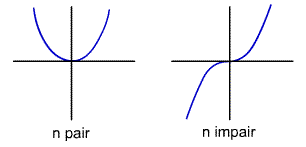
\includegraphics[scale=0.225]{images/008.png} \end{wrapfigure}

Dans un tel tableau la méthode de Karnaugh consiste à rechercher des rectangles dont les dimensions sont des puissances de 2 et dans lesquels la fonction vaut 1 partout.\\\\

Pour le rectangle vert les variables b,c,e prennent les valeurs 0 et 1 alors que les variables a et d sont fixes, les mintermes correspondants peuvent être simplifiés en le simple terme $\neg$a$\wedge$d.\bigskip

Pour le rectangle orange il faut penser à la propriété de tore du tableau. Les variables c et d prennent toutes les valeurs possibles alors que a,b,e sont fixes, le terme obtenu est donc a$\wedge\neg$b$\wedge\neg$e.\\

Pour le rectangle jaune on procède comme pour l'orange (on peut le prolonger sur le vert) : les variables a, c et e sont fixes alors que b et d varient, le terme obtenu est donc $\neg$a$\wedge$c$\wedge\neg$e.\\

Les rectangles violet et rouge ne sont pas simplifiables, on conserve les mintermes initiaux a$\wedge$b$\wedge\neg$c$\wedge\neg$d$\wedge$e et a$\wedge$b$\wedge$c$\wedge$d$\wedge$e.\\

Ainsi la fonction s’écrit en forme normale disjonctive (disjonction de conjonction) comme\\
($\neg$a$\wedge$d)$\vee$(a$\wedge\neg$b$\wedge\neg$e)$\vee $($\neg$a$\wedge$c$\wedge\neg$e)$\vee $(a$\wedge$b$\wedge\neg$c$\wedge\neg$d$\wedge$e)$\vee $(a$\wedge$b$\wedge$c$\wedge$d$\wedge$e).\\

\subsection{Code de Gray} \label{gray}
On va ici regarder comment déterminer le code de Gray.

\subsubsection{De Binaire vers Gray}
Soit un nombre en binaire b $b_{n-1}b_{n-2}...b_{1}b_{0}$.\\

Pour déterminer le code de Gray du numéro correspondant (en ajoutant 1, en effet on commence la numérotation à 0), on garde le bit de poids fort et on obtient chaque bit suivant en effectuant un x-or entre le bit que l'on cherche et celui à sa gauche.\\

Ainsi le b+1$^{\text{ième}}$ nombre de grey est $g=b_{n-1}(b_{n-2}\oplus b_{n-1})...(b_{0}\oplus b_{1})$.\\

\textit{Exemple :}\\
On cherche le 10$^{e}$ nombre de Gray, on prend b=1001. On obtient ainsi g=1101.

\subsubsection{De Gray vers binaire}
Soit un nombre de Gray g $g_{n-1}g_{n-2}...g_{1}g_{0}$.\\

Pour déterminer le numéro de ce code de Gray, on garde le bit de poids fort et on obtient chaque bit suivant en effectuant un x-or entre le bit que l'on cherche et le bit codé à sa gauche.\\

Ainsi g est le $g_{n-1}(b_{n-1}\oplus g_{n-2})...(b_{1}\oplus g_{0})$+1$^{\text{ième}}$ nombre de Gray.\\

\textit{Exemple :}\\
On veut savoir quel nombre de Gray est 1001. On obtient 1110 donc 1001 est le $14+1=15^{\text{ième}}$ code de Gray.





























\end{document}